\chapter{Dziewulscy Gomułowie herbu Rawicz z~Dziewul}

% Przednia okładka podrozdziału
\includepdf{Dziewule_mapa_fin.png}

\section{Dziewule: 1441~r. - 1714~r.}

Prapoczątki rodziny Gomulskich należy prawdopodobnie wiązać z~ziemią 
łukowską, a~konkretnie ze wsią szlachecką Dziewule, która była siedzibą rodu 
Dziewulskich herbu Rawicz. Wieś Dziewule leży nad rzeką Zbuczynką, oddalona 
jest o~około 15~kilometrów na północ od Łukowa i~około 20~kilometrów na 
południowy wschód od Siedlec. Najstarsza znana wzmianka o~Dziewulach pochodzi 
z~1441~roku - wieś ta została wymieniona w~spisanej w~Łukowie umowie 
kupna-sprzedaży wsi Grodzisk oraz Sobiestan - wskazano tam, iż wsie, których 
dotyczyła transakcja, leżą pomiędzy: Zbuczynem, Jasionką i~Dziewulami 
\cite{skuras}. W~połowie XVI~wieku właścicielem folwarku Dziewule był 
Andrzej Dziewulski, wieś tę zamieszkiwali pracujący na folwarku chłopi oraz 
drobna szlachta zagrodowa wywodząca się z~rodu Dziewulskich, o~następujących 
przydomkach: Markowicz, Górny, Dziecinka i~Starczowicz \cite{eszeliga} - 
szlachta, dla której w~rejestrach poborowych jest wskazane, iż \enquote{nie 
posiada kmieci} oraz \enquote{sama orze} \cite{aboczek}.

\begin{figure}[!ht]
    \vspace*{0.6cm}
    \centering 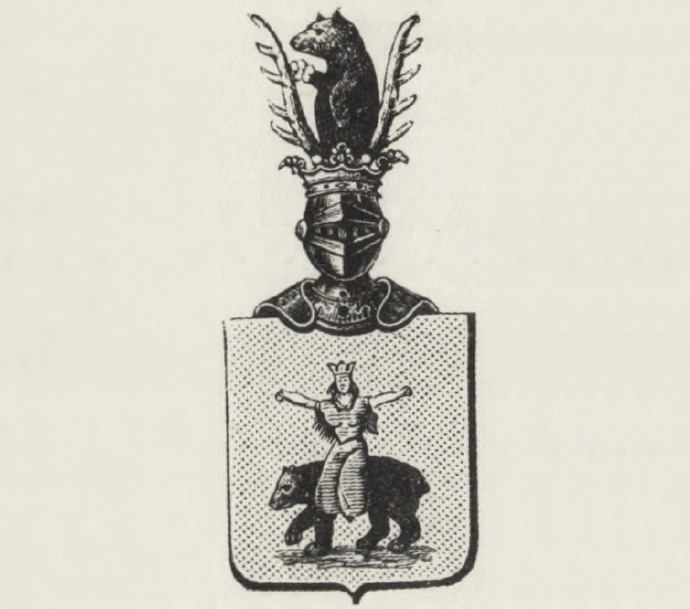
\includegraphics[width=1.0\linewidth]{Herb_Rawicz_1902.png}
    \captionsetup{format=hang}
    \caption{Rawicz - herb rodziny Dziewulskich z~Dziewul zamieszczony 
    w~piątym tomie \emph{Herbarza Polskiego} Adama Bonieckiego 
    \cite{aboniecki}.}
    \label{fig:dziewulscy_herb}
\end{figure}

Dlaczego podane wyżej informacje są istotne z~perspektywy historii rodziny 
Gomulskich? Gdyż na przełomie XVII~wieku i~XVIII~wieku, w~rejestrach 
pogłównego województwa lubelskiego \cite{agad1} oraz w~aktach stanu cywilnego 
parafii rzymskokatolickiej w~Zbuczynie, we wsi Dziewule pojawiają się 
Dziewulscy o~przydomkach: \textbf{Gomuła}, \textbf{Gomolik}, \textbf{Gomolak} 
oraz \textbf{Gomoła}, a~jak pokażę w~dalszej części niniejszej książki, to 
właśnie z~tych przydomków prawdopodobnie w~kolejnych pokoleniach wykształciło 
się nazwisko Gomulski. Wyżej wymienione przydomki etymologicznie można 
natomiast wywodzić od słów  \emph{gomuła} / \emph{gomoła}, które 
w~staropolszczyźnie oznaczały łysego byka jelenia tuż po zrzuceniu 
poroża\footnote{Słowo \emph{gomóła} / \emph{gomuła} funkcjonuje do dzisiaj 
pod tym znaczeniem w~żargonie myśliwskim.} oraz okrągłą porcję białego sera.

\begin{figure}[!ht]
    \centering
    \subfloat{{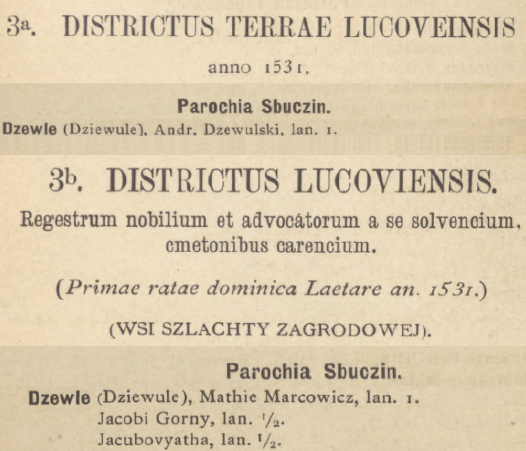
\includegraphics[width=0.55\linewidth]{Dziewule_1531.png}}}
    \qquad
    \subfloat{{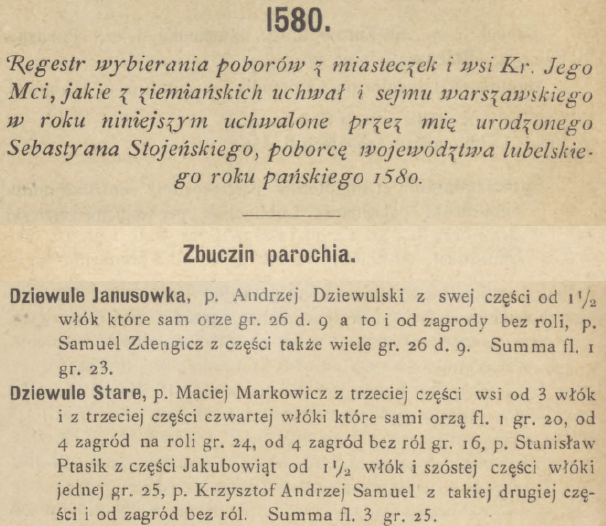
\includegraphics[width=0.55\linewidth]{Dziewule_1580.png}}}
    \caption{Wpisy dotyczące wsi Dziewule pochodzące z~rejestrów poborowych 
    województwa lubelskiego sporządzonych w~1531~roku oraz 1580~roku 
    \cite{apawinski}.}
    \label{fig:dziewule_1531_1580}
\end{figure}

Tworzenie się przydomków wśród drobnej szlachty zagrodowej było powszechną 
praktyką w~tamtych czasach, pojawiały się one ze względu na potrzebę 
rozróżnienia członków rodziny o~tych samych imionach, pochodzących z~tej 
samej miejscowości. W~przypadku rodziny Dziewulskich herbu Rawicz 
zamieszkującej wieś Dziewule, już w~XVI wieku, tak jak wcześniej wspominano, 
część rodziny zaczęła posługiwać się przydomkami Markowicz, Górny, Dziecinka 
czy Starczowicz. W~XVII~wieku, w~skutek dalszego intensywnego rozrostu 
rodziny Dziewulskich na terenie Dziewul, konieczne stało się wykształcenie 
nowych przydomków. Marek Woliński w~swojej książce \emph{Herbarz szlachty 
ziemi łukowskiej na Lubelszczyźnie. Tom III} wymienia następujące przydomki 
Dziewulskich herbu Rawicz: Dziecinka, Garbaciak, Garbaczyk, 
\textbf{Gomolak}, \textbf{Gomolik}, \textbf{Gomoła}, \textbf{Gomuła}, Górny, 
Grabarczyk, Jakubowięta, Jaroszczyk, Jaroszy, Jedynak, Jędrzejowięta, 
Kosiorek, Kozieranek, Kwasek, Leszczyk, Maraszczyk, Markowicz, Maroszczyk, 
Mizerak, Piotrowicz, Piskiel, Ptasik, Ptaszkowicz, Pyskiel, Pyskowicz, 
Siestrzeniec, Starczowicz, Starczyk, Staroszczyk, Starzeł, Starzec, 
Synowczyk, Szymończyk, Tarczyniak, Turczyniak, Zdengicz \cite{wolinski}. 
Przydomki rodzin drobnoszlacheckich często stawały się w~kolejnych 
pokoleniach ich nazwiskami, szczególnie gdy dana rodzina opuszczała 
miejscowość związaną ze swoim nazwiskiem w~skutek utraty własności ziemi, 
ubożała i~ze stanu szlacheckiego była degradowana do stanu chłopskiego. Ten 
proces został dobrze opisany przez Marka Wolińskiego, w~przytaczanym już tu 
wcześniej herbarzu:

\begin{quote}{Marek Woliński \\ \null\hfill \emph{Herbarz szlachty ziemi 
    łukowskiej na Lubelszczyźnie. Tom III} \\ \null\hfill (str. 38-41, 
    wyd. 1)}
\textit{Niezależnie od opisanych przykładów przejście do nazwisk 
o~charakterze przydomkowym dotyczyło drobnej szlachty, a~presji w~tym 
kierunku towarzyszyło ubożenie, aż do momentu krytycznego, którym była walka 
o~zachowanie lub wyzbycie się \enquote{ostatniej} cząstki posiadanej 
nieruchomości. Cząstką tą była ziemia. \enquote{Ostatnia} cząstka to ta, 
której dalszy podział kreuje już tylko grządki, których uprawa pozbawia 
właściciela możliwości płacenia podatku, jednocześnie nie zaspokajając 
żadnej życiowej potrzeby. W~takiej sytuacji potrzeby życiowe zmuszają nawet 
najbardziej szlachetnego właściciela do stania się najmitą, a~szlacheckość 
pochodzenia zostaje zepchnięta w~przeszłość. Teraźniejszość zostaje ze 
szlachectwa ogołocona.
\\
\\
(...)
\\
\\
Przekonujemy się z~łatwością, że zmiana podmiotowego i~społecznego położenia 
nie była niczym nadzwyczajnym w~praktyce życia społeczności lokalnych. 
Wykluczona była sytuacja, w~której zmiana takiego położenia byłaby związane 
z~jakimś precedensem. Nie była więc to jakaś podróż w~nieznane. Wiedziano, 
że istnieje taka możliwość, że jedynym może się poszczęścić, a~drugich 
spotkać ruina. Istnienie Marchewków, całkowicie zubożałych Krasuskich, bez 
swego szlacheckiego przedstawiciela w~XVIII~wieku, w~kręgu swych szlacheckich 
krewniaków, nie świadczy o~jakiś radykalnych elementach wykluczenia 
i~istnieniu murów klasowych. Po prostu, jak się wydaje, odmieniały się losy 
i~bieg spraw życiowych wyglądał inaczej, ale przyjaźnie i~więzi społeczne 
pozostawały. Tylko jednostki, może co bardziej ambitne czy dumne, a~może po 
prostu odważne, zaczynały wszystko od nowa gdzieś indziej.}
\end{quote}

\begin{figure}[!ht]
    \vspace*{0.5cm}
    \centering 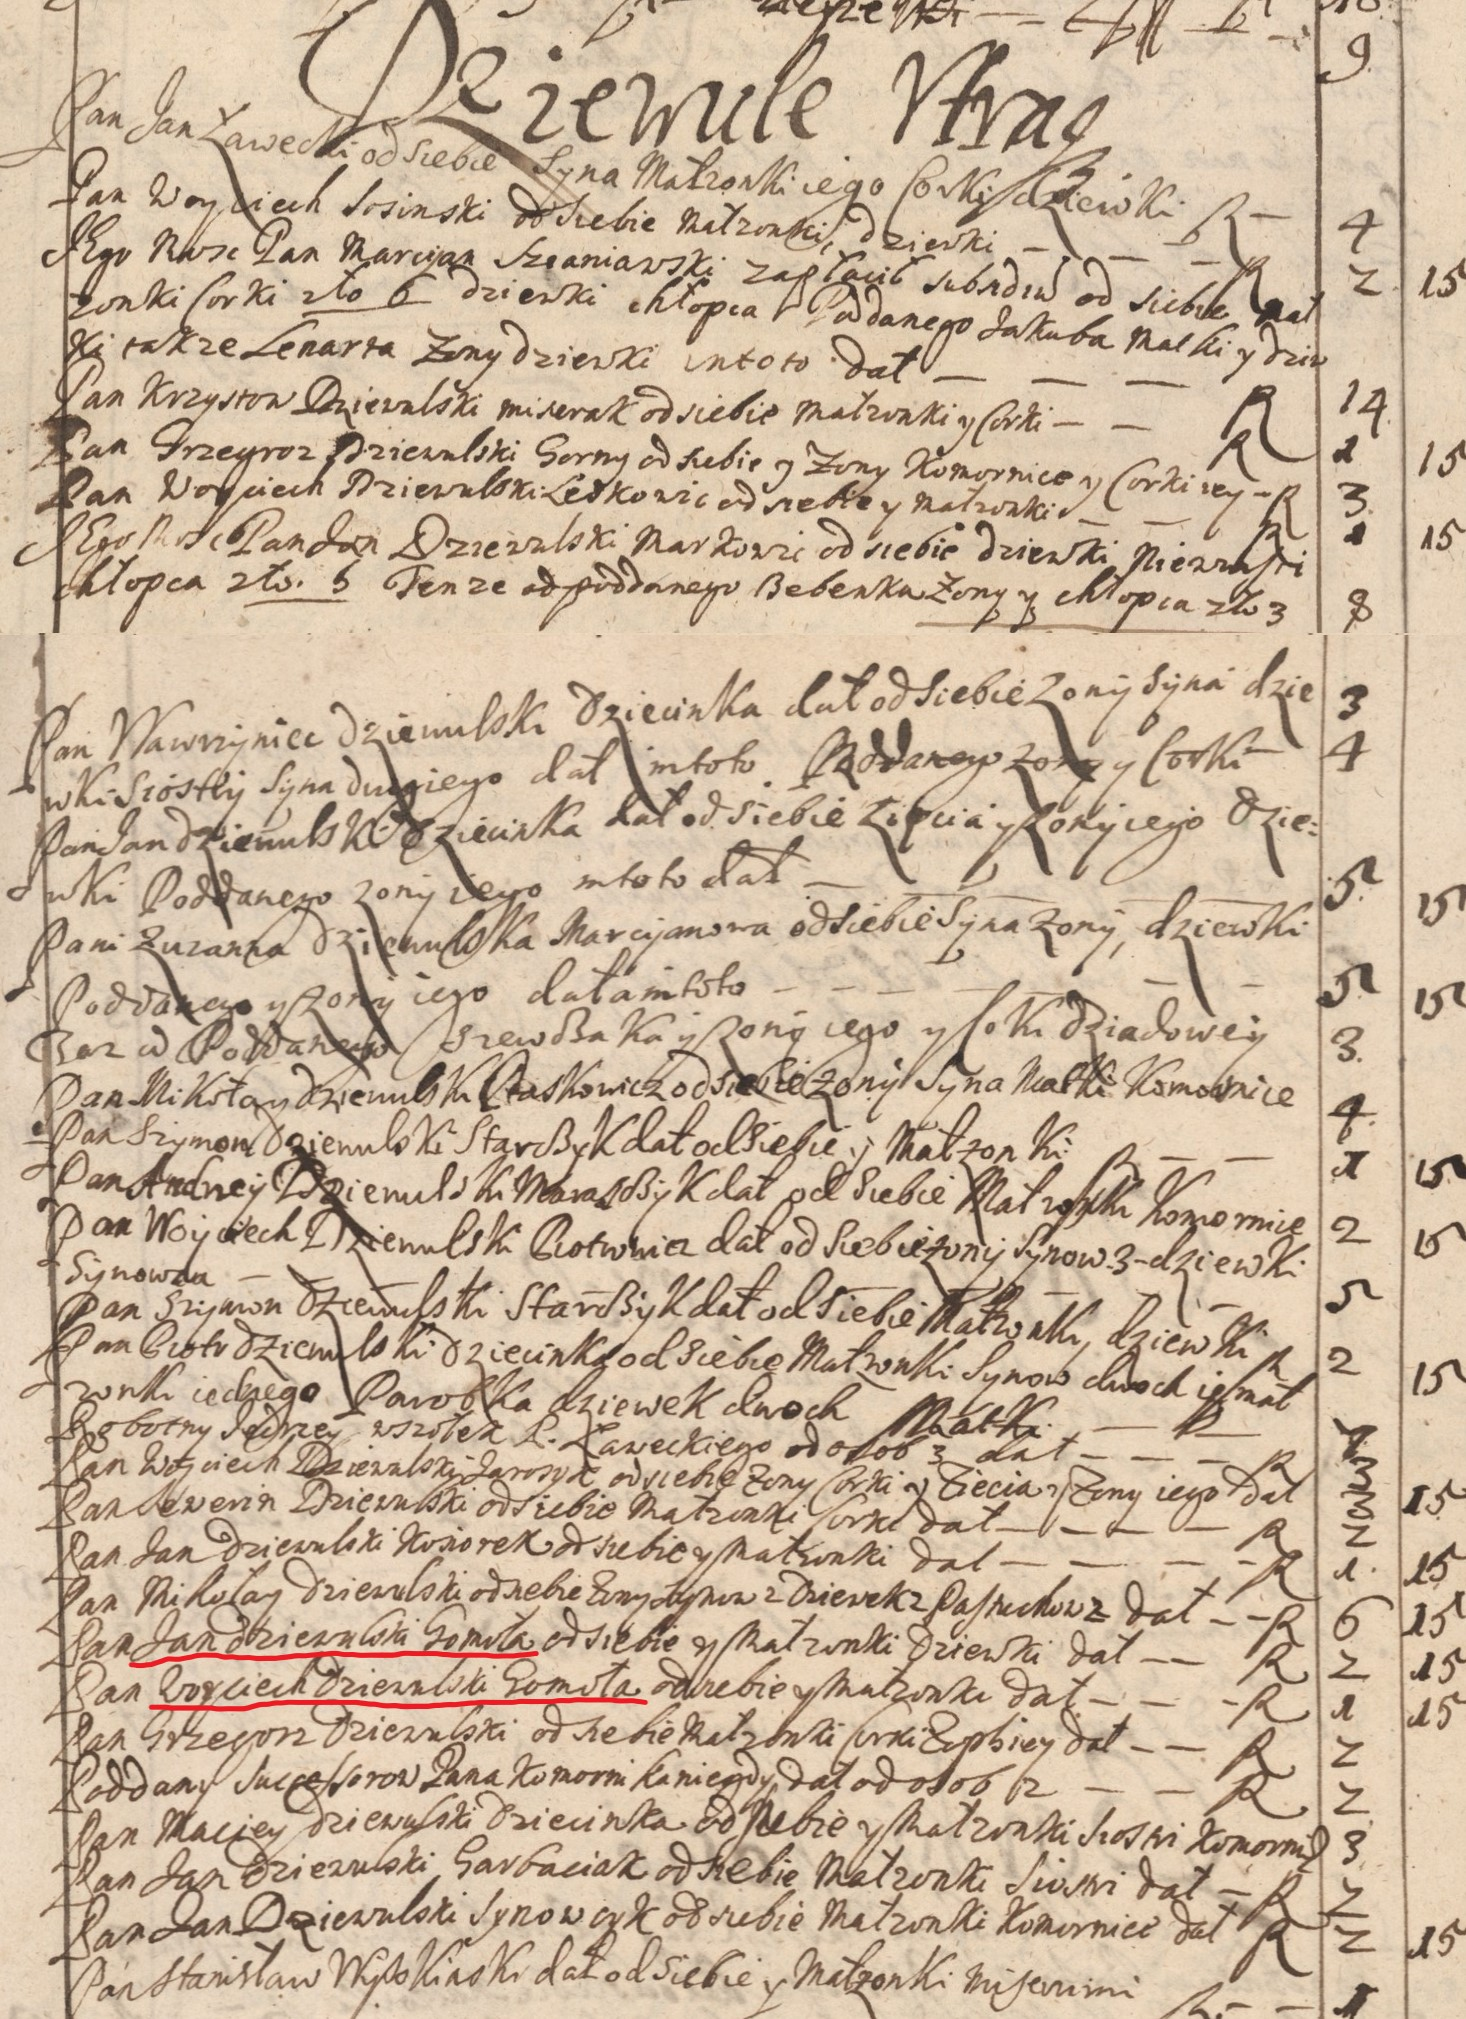
\includegraphics[width=0.9\linewidth]{
        Rejestry_pogłównego_generalnego_Dziewule_1673_Gomoła_sygn_1_7_0_3_72.jpg}
    \captionsetup{format=hang}
    \caption{Fragment rejestru pogłównego województwa lubelskiego dla wsi 
    Dziewule z~1673 roku - na czerwono podkreślono wpisy dotyczące Jana 
    Dziewulskiego Gomuła oraz Wojciech Dziewulskiego Gomuła \cite{agad1}.}
    \label{fig:dziewule_1673}
\end{figure}

Rejestr pogłównego województwa lubelskiego dla wsi Dziewule z~1673 roku 
(patrz: ryc. \ref{fig:dziewule_1673}) spośród 23~szlachciców o~nazwisku 
Dziewulski, dwóch określa dodatkowo przydomkiem \textbf{Gomuła}:
\begin{itemize}
\item \textit{Pan Jan Dziewulski \textbf{Gomuła} od siebie i~małżonki, 
dziewki dał - razem: 2 | 15},
\item \textit{Pan Wojciech Dziewulski \textbf{Gomuła} od siebie i~małżonki 
dał - razem: 1 | 15}.
\end{itemize}

\begin{figure}[!ht]
    \vspace*{0.5cm}
    \centering 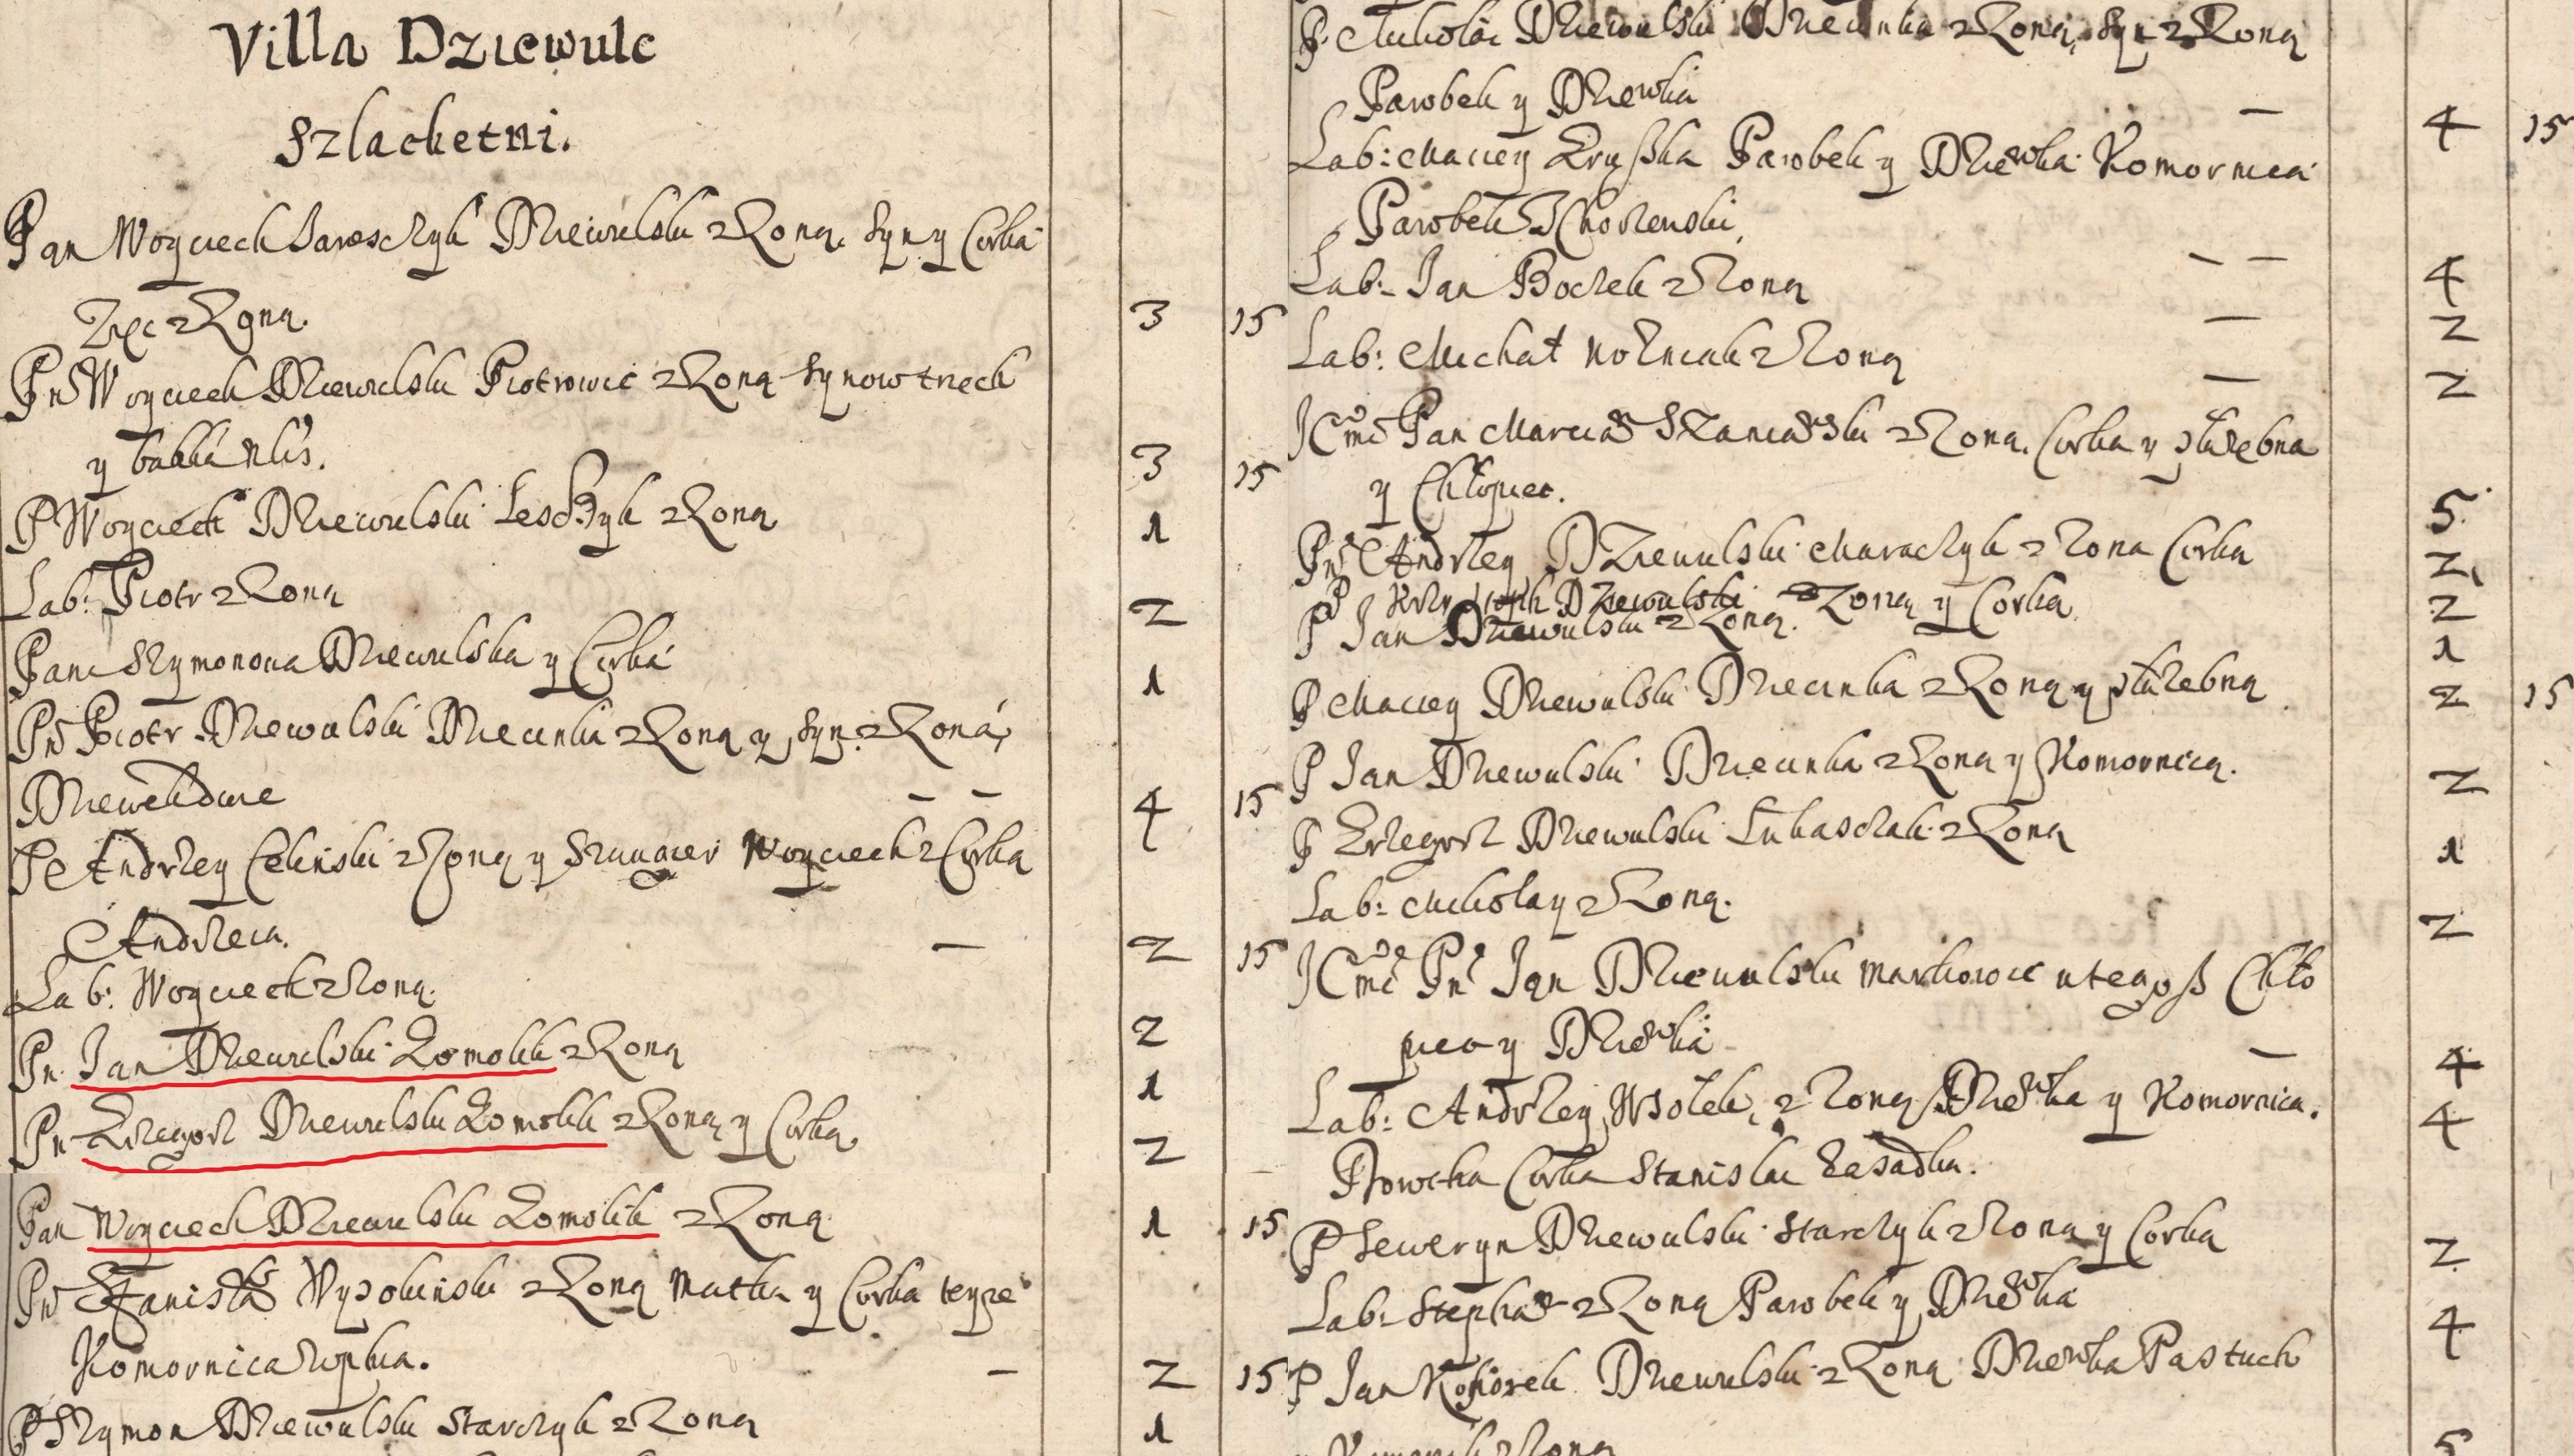
\includegraphics[width=1.0\linewidth]{
        Rejestry_pogłównego_generalnego_Dziewule_1674_Gomolik_sygn_1_7_0_3_72.jpg}
    \captionsetup{format=hang}
    \caption{Fragment rejestru pogłównego województwa lubelskiego dla wsi 
    Dziewule z~1674 roku - na czerwono podkreślono wpisy dotyczące Jana 
    Dziewulskiego Gomolika, Wojciech Dziewulskiego Gomolika oraz Grzegorza 
    Dziewulskiego Gomolika \cite{agad1}.}
    \label{fig:dziewule_1674}
\end{figure}

Rejestr z~kolejnego roku (patrz: ryc. \ref{fig:dziewule_1674}) wymienia trzy 
osoby o~przydomku \textbf{Gomolik} - są to ponownie Jan i~Wojciech, ale także 
Grzegorz, który, być może omyłkowo, w~poprzednim spisie znalazł się bez 
przydomku (\enquote{Pan Grzegorz Dziewulski od siebie, małżonki, córki dał - 
razem: 2}):
\begin{itemize}
\item \textit{Pan Jan Dziewulski \textbf{Gomolik} z~żoną: 1},
\item \textit{Pan Grzegorz Dziewulski \textbf{Gomolik} z~żoną i~córka: 2},
\item \textit{Pan Wojciech Dziewulski \textbf{Gomolik} z~żoną: 1 | 15}.
\end{itemize}

Rejestr z~1676~roku (patrz: ryc. \ref{fig:dziewule_1676}) ponownie wymienia 
trzy osoby o~przydomku \textbf{Gomolik}, są to Jan, Wojciech i~Grzegorz, ale 
tym razem nie podaje ich nazwiska rodowego (pomimo, iż dla niektórych osób 
podane jest zarówno nazwisko rodowe, jak i~przydomek np. \enquote{Jan 
Dziewulski Dziecinka}):

\begin{itemize}
\item \textit{Szlachetny Jan \textbf{Gomolik} z~żoną: 3},
\item \textit{Szlachetny Grzegorz \textbf{Gomolik} z~córką, 
sprzężajem robi: 2},
\item \textit{Szlachetny Wojciech \textbf{Gomolik} z~żoną, komornic 2., 
które wyrabiają: 6}.
\end{itemize}

\begin{figure}[!ht]
    \vspace*{0.5cm}
    \centering 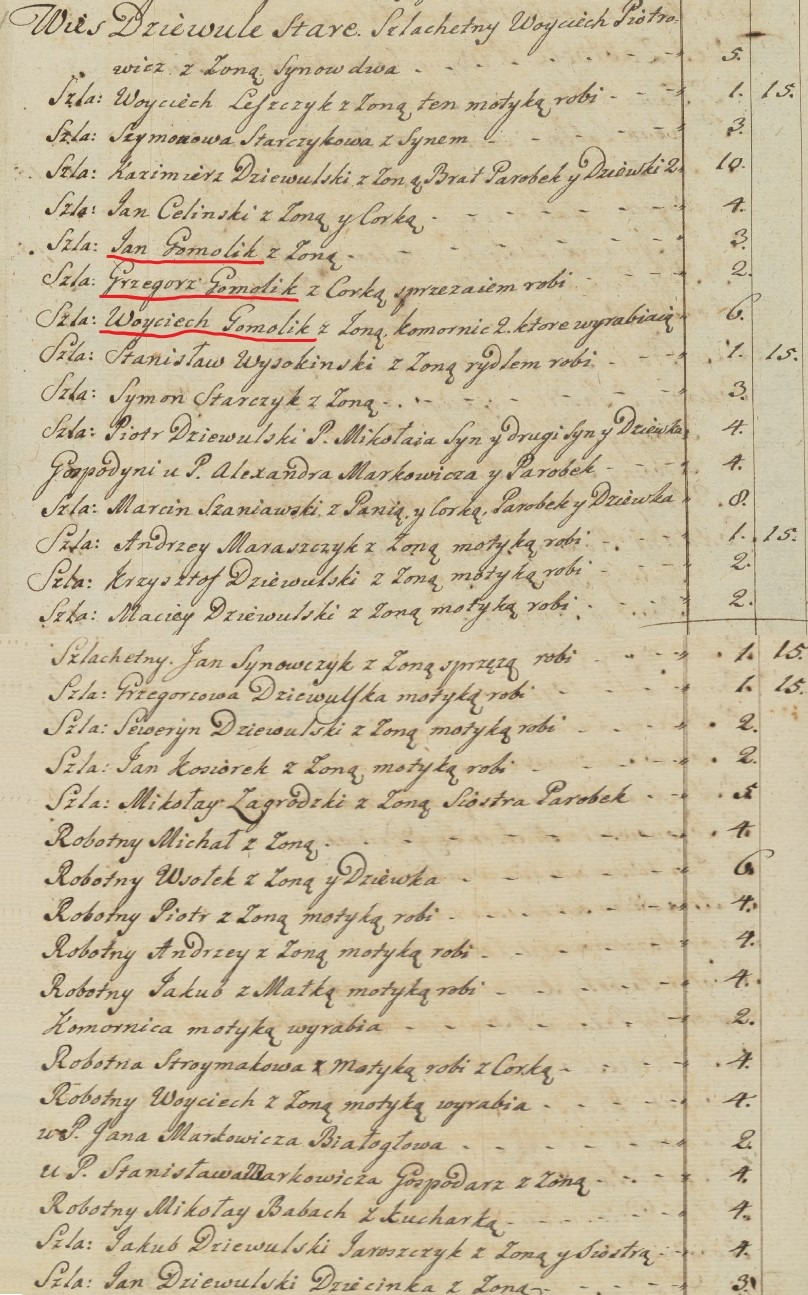
\includegraphics[width=0.8\linewidth]{
        Rejestry_pogłównego_prowincyi_małopolskiey_Dziewule_1676_Gomolik_2.jpg}
    \captionsetup{format=hang}
    \caption{Fragment rejestru pogłównego \enquote{prowincyi małopolskiey} 
    dla wsi Dziewule Stare z~1676 roku - na czerwono podkreślono wpisy 
    dotyczące Jana Gomolika, Wojciecha Gomolika oraz Grzegorza Gomolika 
    \cite{floyko}.}
    \label{fig:dziewule_1676}
\end{figure}

Na przykładzie tych rejestrów można zobaczyć jak swobodnie podchodzono 
w~tamtych czasach do zapisywania nazwisk i~przydomków w~oficjalnych 
dokumentach - przydomek, który w~jednym z~rejestrów był zapisywany jako 
\enquote{Gomuła} w~kolejnym zmieniał się w~\enquote{Gomolika}. Nie zachowały 
się niestety do dnia dzisiejszego inne rejestry pogłównego dla wsi Dziewule 
z~przełomu XVII~i~XVIII~wieku. Z~dostępnych obecnie źródeł warto przyjrzeć 
się aktom chrztów w~parafii rzymskokatolickiej pod wezwaniem św.~Stanisława 
Biskupa Męczennika i~Aniołów Stróżów w~Zbuczynie dla lat 
1702-1749\footnote{Akta te dostępne są w~formie cyfrowej na portalu 
\emph{szukajwarchiwach.gov.pl}, pod adresem: \\ 
\url{https://www.szukajwarchiwach.gov.pl/en/zespol/-/zespol/56418} (dostęp: 
marzec 2024 r.).}. W~aktach tych znajdziemy wprawdzie jedynie informacje 
o~rodzinach, w~których rodziły się w~tamtych latach dzieci, ale to też bardzo 
wartościowe źródło informacji.

\begin{figure}[!ht]
    \vspace*{0.5cm}
    \centering 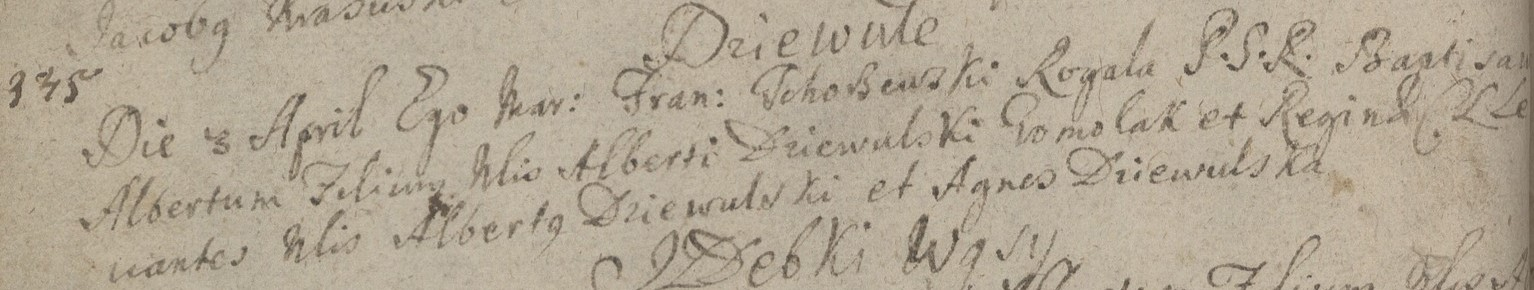
\includegraphics[width=1.0\linewidth]{
        1702_Wojciech_Gomolak_Dziewulski_akt_narodzin_parafia_Zbuczyn_wpis_345.jpg}
    \captionsetup{format=hang}
    \caption{Akt chrztu Wojciech Dziewulskiego Gomolaka - par. Zbuczyn 
    1702~rok (345/1702-1714) \cite{par_zbuczyn1}.}
    \label{fig:wgomola_1702}
\end{figure}

\begin{figure}[!ht]
    \vspace*{0.5cm}
    \centering 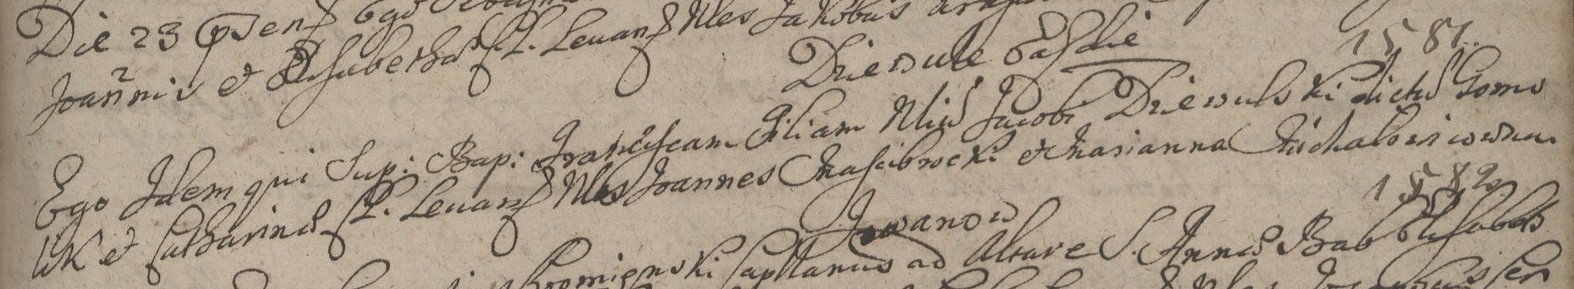
\includegraphics[width=1.0\linewidth]{
        1706_Franciszka_Gomolik_Dziewulski_akt_narodzin_parafia_Zbuczyn_wpis_1587.jpg}
    \captionsetup{format=hang}
    \caption{Akt chrztu Franciszki Dziewulskiej Gomolik - par. Zbuczyn 
    1706~rok (1587/1702-1714) \cite{par_zbuczyn1}.}
    \label{fig:fgomola_1706}
\end{figure}

Z~akt parafii w~Zbuczynie wynika, że w~latach 1702-1730 w~Dziewulach urodziło 
się około 120~osób o~nazwisku Dziewulski, co potwierdza hipotezę o~szybkim 
rozroście rodziny Dziewulskich na przełomie 
XVII~i~XVIII~wieku\footnote{Rejestry pogłówne z~lat 1673-1676 wskazują, że 
jeszcze w~latach 70. XVII~wieku w~Dziewulach mieszkało około 50~osób 
o~nazwisku Dziewulski.}. Czwórka spośród tych 120~nowo narodzonych dzieci 
miała ojca posługującego się przydomkiem Gomolak / Gomolik / Gomoła, były to:

\begin{itemize}
\item Wojciech (łac. \emph{Albertum}) urodzony w~1702~roku ze szlachetnych 
Wojciecha Dziewulskiego \textbf{Gomolaka} i~Reginy, którego rodzicami 
chrzestnymi zostali szlachetni Wojciech oraz Agnieszka Dziewulscy (patrz: 
ryc. \ref{fig:wgomola_1702}),
\item Franciszka (łac. \emph{Franciscam}) urodzona w~1706~roku ze 
szlachetnych Jakuba Dziewulskiego \textbf{Gomolika} i~Katarzyny, której 
rodzicami chrzestnymi zostali szlachetni Jan Maścibrocki oraz Marianna 
Michałowska (patrz: ryc. \ref{fig:fgomola_1706}),
\item Franciszek (łac. \emph{Franciscum}) urodzony w~1722~roku ze 
szlachetnych Antoniego \textbf{Gomoła} Dziewulskiego i~Katarzyny, którego 
rodzicami chrzestnymi zostali Mateusz Choynowski oraz Zofia Przesmycka 
(patrz: ryc. \ref{fig:fgomola_1722}),
\item Marianna (łac. \emph{Mariannam}) urodzona w~1727~roku ze szlachetnych 
Stanisława Dziewulskiego \textbf{Gomolaka} i~Rozalii, której rodzicami 
chrzestnymi zostali szlachetni Marcin Grodzicki oraz Marianna Dziewulska 
(patrz: ryc. \ref{fig:mgomola_1727}).
\end{itemize}

Warto zwrócić uwagę, iż w~akcie chrztu Franciszka Gomoła Dziewulskiego jego 
rodzice chrzestni nie są określeni tytułem szlachetnych (łac. \emph{Noblis}, 
skrót - \emph{Nls.}) tak jak jego rodzice, co oznacza, iż prawdopodobnie 
pochodzili z~niższej warstwy społecznej, co mogłoby sugerować pewne zubożenie 
tej gałęzi rodziny Dziewulskich\footnote{W~tamtym czasie w~ziemi łukowskiej 
dosyć często praktykowany był zwyczaj, iż rodzicami chrzestnymi chłopa byli 
szlachcice, ale sytuacje odwrotne były raczej incydentalne, gdyż rodzicom 
nowo narodzonego dziecka bardzo zależało, żeby rodzicami chrzestnymi ich 
dzieci zostawały jak najbardziej majętne osoby, co miało im pomóc w~dalszym 
życiu.}. 

\begin{figure}[!ht]
    \vspace*{0.5cm}
    \centering \includegraphics[width=1.0\linewidth]{
        1722_Franciszek_Gomoła_Dziewulski_akt_narodzin_parafia_Zbuczyn_wpis_1589.jpg}
    \captionsetup{format=hang}
    \caption{Akt chrztu Franciszka Gomoła Dziewulskiego - par. Zbuczyn 
    1722~rok (1589/1714-1729) \cite{par_zbuczyn2}.}
    \label{fig:fgomola_1722}
\end{figure}

\begin{figure}[!ht]
    \vspace*{0.5cm}
    \centering 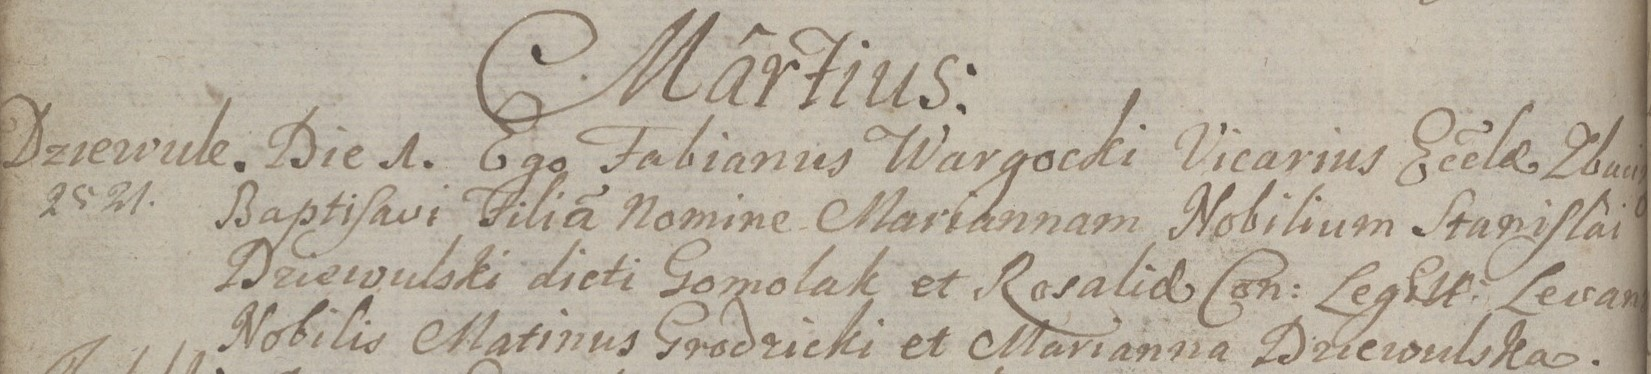
\includegraphics[width=1.0\linewidth]{
        1727_Marianna_Gomolak_Dziewulska_akt_narodzin_parafia_Zbuczyn_wpis_2521.jpg}
    \captionsetup{format=hang}
    \caption{Akt chrztu Marianny Dziewulskiej Gomolak - par. Zbuczyn 1727~rok 
    (2521/1714-1729) \cite{par_zbuczyn2}.}
    \label{fig:mgomola_1727}
\end{figure}

W~związku z~tym, iż akta chrztu w~tamtych czasach spisywane były po łacinie, 
w~sposób niezwykle lakoniczny (spisujący je księża często stosowali skróty 
typu \emph{No.} zamiast \emph{Nomine} czy \emph{Nls.} zamiast \emph{Noblis}), 
często zdarzało się, że duchowny tworzący wpis nie dopisywał przydomka przy 
nazwisku ojca. Dlatego warto prześledzić inne wpisy, w~których jako rodzice 
pojawiają się Wojciech i~Regina Dziewulscy, Jakub i~Katarzyna Dziewulscy, 
Antoni i~Katarzyna Dziewulscy czy Stanisław i~Rozalia Dziewulscy. W~ten 
sposób odnaleźć można w~Dziewulach jeszcze trójkę dzieci urodzonych w~latach 
1702-1730, które prawdopodobnie odziedziczyły przydomki Gomolik / Gomoła:

\begin{itemize}
\item Maciej (łac. \emph{Mathiam}) urodzony w~1703~roku ze szlachetnych 
Jakuba Dziewulskiego \textbf{Gomolika} i~Katarzyny, którego rodzicami 
chrzestnymi zostali szlachetni Wojciech oraz Regina Dziewulscy Gomolakowie 
(patrz: ryc. \ref{fig:mgomola_1703}),
\item Marianna (łac. \emph{Mariannam}) urodzona w~1714~roku ze szlachetnych 
Antoniego \textbf{Gomoła} Dziewulskiego i~Katarzyny, której rodzicami 
chrzestnymi zostali szlachetni Wojciech Radomyski oraz Marianna Dziewulska 
(patrz: ryc. \ref{fig:mgomola_1714}),
\item Wojciech (łac. \emph{Adalbertum}) urodzony w~1725~roku ze szlachetnych 
Antoniego \textbf{Gomoła} Dziewulskiego i~Katarzyny, którego rodzicami 
chrzestnymi zostali szlachetni Wojciech oraz Katarzyna Dziewulscy 
(patrz: ryc. \ref{fig:wgomola_1725}).
\end{itemize}

Mamy więc finalnie siedmioro dzieci należących do odłamu rodziny Dziewulskich 
posługujących się przydomkiem Gomolak / Gomolik / Gomoła / Gomuła, z~czego 
czwórka z~nich to chłopcy, którzy, o~ile założyli własne rodziny, mogli 
przekazać ten przydomek następnym pokoleniom. Dwóch z~tych chłopców dostało 
na chrzcie imię Wojciech, co utrudnia śledzenie ich dalszych losów, gdyż było 
to najpopularniejsze imię męskie w~tamtych czasach. W~samych tylko 
Dziewulach, w~latach 1702-1749, mieszkało co najmniej 10~rodzin, w~których 
ojcowie mieli na imię Wojciech (z~przydomkami: Gomolak, Gomoła, Jedynak, 
Synowczyk, Garbaczyk), z~łącznie około 70~rodzin zamieszkujących Dziewule na 
początku XVII~wieku.

\begin{figure}[!ht]
    \vspace*{0.5cm}
    \centering 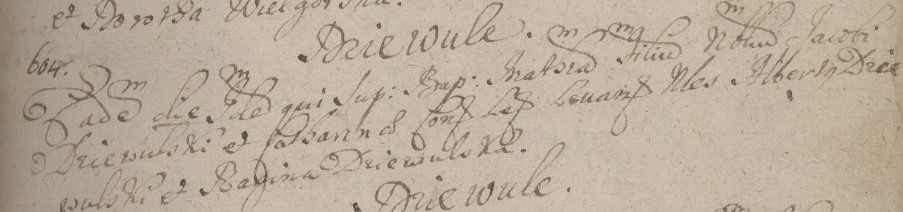
\includegraphics[width=1.0\linewidth]{
        1703_Maciej_Gomolik_Dziewulski_akt_chrztu_parafia_Zbuczyn_wpis_604.jpg}
    \captionsetup{format=hang}
    \caption{Akt chrztu Macieja Dziewulskiego Gomolika - par. Zbuczyn 
    1703~rok (604/1702-1714) \cite{par_zbuczyn1}.}
    \label{fig:mgomola_1703}
\end{figure}

\begin{figure}[!ht]
    \vspace*{0.5cm}
    \centering \includegraphics[width=1.0\linewidth]{
        1714_Marianna_Gomoła_Dziewulska_akt_chrztu_parafia_Zbuczyn_wpis_32.png}
    \captionsetup{format=hang}
    \caption{Akt chrztu Marianny Dziewulskiej Gomoły - par. Zbuczyn 1714~rok 
    (32/1714-1729) \cite{par_zbuczyn1}.}
    \label{fig:mgomola_1714}
\end{figure}

Z~dalszej analizy akt parafii w~Zbuczynie wynika, że po 1730~roku, przez 
kolejne 20~lat, w~Dziewulach urodziło się już tylko około 40~osób o~nazwisku 
Dziewulski i~ojciec żadnego z~urodzonych dzieci nie został wskazany w~aktach 
parafii jako Gomolak / Gomolik / Gomoła / Gomuła. Na podstawie analizy 
akt~parafialnych możemy jednak stwierdzić, iż Maciej Dziewulski Gomolik 
(syn Jakuba i~Katarzyny) wspólnie z~żoną Ewą miał dwie córki urodzone 
w~Dziewulach przed 1750 rokiem: Jadwigę (ur. 1728~r. - patrz ryc. 
\ref{fig:jgomola_1728}) oraz Ewę (ur. 1731~r. - patrz ryc. 
\ref{fig:egomola_1731}), natomiast Wojciech Dziewulski Gomoła (syn Antoniego 
i~Katarzyny) razem z żoną Agnieszką mieli jedną córkę urodzoną w~Dziewulach 
przed 1750 rokiem - tą córką była Elżbieta (ur. 1748~r. - patrz ryc. 
\ref{fig:egomola_1748}). Franciszek Dziewulski Gomoła (syn Antoniego 
i~Katarzyny) oraz Wojciech Dziewulski Gomolak (syn Wojciecha i Reginy) nie 
pojawiają się jako rodzice żadnego dziecka urodzonego w~Dziewulach w~latach 
1702-1749, więc być może nie dożyli wieku dorosłego, nie założyli własnej 
rodziny lub opuścili rodzinną wieś.

\begin{figure}[!ht]
    \vspace*{0.5cm}
    \centering \includegraphics[width=1.0\linewidth]{
        1725_Wojciech_Gomoła_Dziewulski_akt_chrztu_parafia_Zbuczyn_wpis_2099.png}
    \captionsetup{format=hang}
    \caption{Akt chrztu Wojciecha Dziewulskiego Gomoły - par. Zbuczyn 
    1725~rok (2099/1714-1729) \cite{par_zbuczyn2}.}
    \label{fig:wgomola_1725}
\end{figure}

\begin{figure}[!ht]
    \vspace*{0.5cm}
    \centering 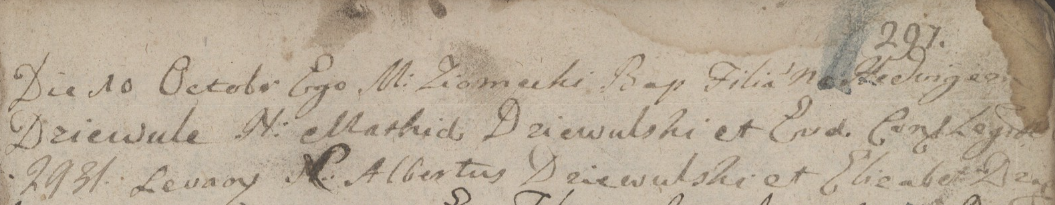
\includegraphics[width=1.0\linewidth]{
        1728_Jadwiga_Gomolik_Dziewulska_akt_chrztu_parafia_Zbuczyn_wpis_2931.png}
    \captionsetup{format=hang}
    \caption{Akt chrztu Jadwigi Dziewulskiej Gomolik - par. Zbuczyn 1728~rok 
    (2931/1714-1729) \cite{par_zbuczyn2}.}
    \label{fig:jgomola_1728}
\end{figure}

\begin{figure}[!ht]
    \vspace*{0.5cm}
    \centering 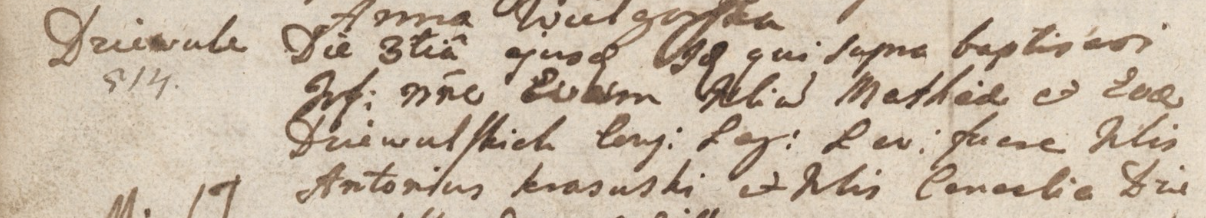
\includegraphics[width=1.0\linewidth]{
        1731_Ewa_Dziewulska_Gomolik_akt_chrztu_parafia_Zbuczyn_wpis_514.png}
    \captionsetup{format=hang}
    \caption{Akt chrztu Ewy Dziewulskiej Gomolik - par. Zbuczyn 1731~rok 
    (514/1729-1749) \cite{par_zbuczyn3}.}
    \label{fig:egomola_1731}
\end{figure}

Akta chrztów parafii w~Zbuczynie z~lat 1750-1764, w~momencie pisania 
niniejszej książki, nie były dostępne w~wersji cyfrowej, niemożliwe było też 
zapoznanie się z~nimi w~parafii, gdyż decyzją tamtejszego biskupa żadne akta 
kościelne w~diecezji siedleckiej, pochodzące z~tak odległych czasów, nie były 
udostępniane osobom prywatnym, gdyż były one \enquote{zbyt cenne 
i~jednostkowe}. W~momencie pisania niniejszej książki dostępne były natomiast 
cyfrowe kopie akt chrztów w~parafii zbuczyńskiej dla lat 1765-1785. W~latach 
tych we wsi Dziewule urodziło się około 40~osób o~nazwisku Dziewulski, co 
ciekawe nie każda osoba urodzona z~tym nazwiskiem pochodziła z~rodziny 
szlacheckiej. Cześć rodziców nowo narodzonych dzieci określana była 
w~metrykach parafialnych jako chłopi (\emph{Laboriosus} w~skrócie 
\emph{Lab.}) - patrz: ryc. \ref{fig:edziewulska_1777}. Dotąd we wszystkich 
dostępnych aktach parafialnych parafii Zbuczyn, z~lat 1702-1749, przed 
nazwiskiem Dziewulski dodawany był zawsze skrót \emph{Nls.} (\emph{Noblis}) 
oznaczający osobę pochodzącą ze stanu szlacheckiego.

\begin{figure}[!ht]
    \vspace*{0.5cm}
    \centering 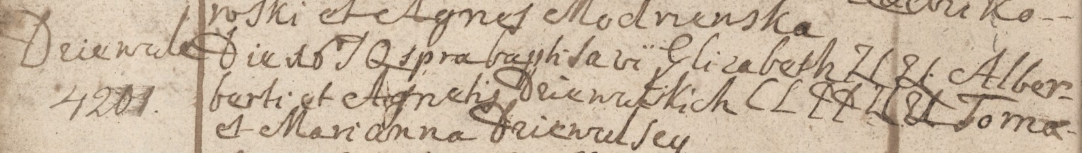
\includegraphics[width=1.0\linewidth]{
        1748_Elżbieta_Dziewulska_Gomoła_akt_chrztu_parafia_Zbuczyn_wpis_4201.png}
    \captionsetup{format=hang}
    \caption{Akt chrztu Elżbiety Dziewulskiej Gomoły - par. Zbuczyn 1748~rok 
    (4201/1729-1749) \cite{par_zbuczyn3}.}
    \label{fig:egomola_1748}
\end{figure}


\begin{figure}[!ht]
    \vspace*{0.5cm}
    \centering 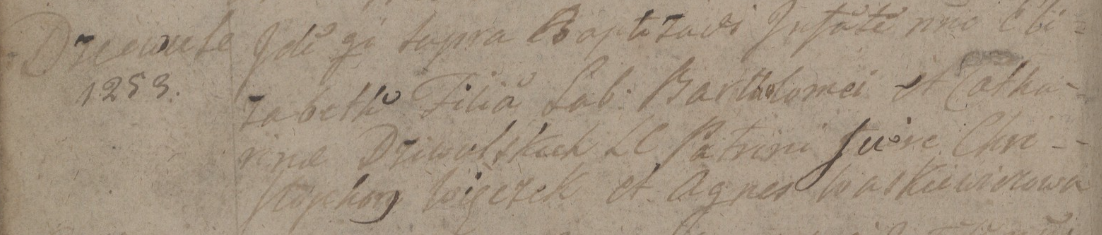
\includegraphics[width=1.0\linewidth]{
        175. 1777_Elżbieta_Dziewulska_córka_LAB_Bartłomieja_Katarzyny.png}
    \captionsetup{format=hang}
    \caption{Akt chrztu chłopki Elżbiety Dziewulskiej - par. Zbuczyn 1777~rok 
    (1253/1773-1781) \cite{par_zbuczyn5}.}
    \label{fig:edziewulska_1777}
\end{figure}

\begin{figure}[!ht]
    \vspace*{0.5cm}
    \centering 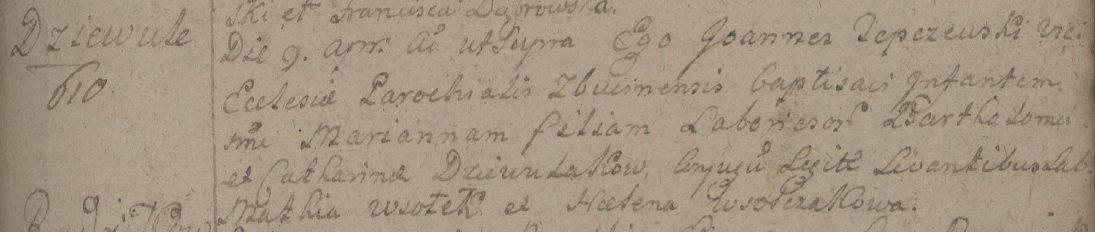
\includegraphics[width=1.0\linewidth]{
        170. 1775_Marianna_Dziewulak_córka_LAB_Bartłomieja_Katarzyny.png}
    \captionsetup{format=hang}
    \caption{Akt chrztu chłopki Marianny Dziewulak - par. Zbuczyn 1775~rok 
    (610/1773-1781) \cite{par_zbuczyn5}.}
    \label{fig:mdziewulak_1775}
\end{figure}

Kolejnym ciekawym zjawiskiem było pojawienie się w~Dziewulach, w~latach 
70.~XVIII wieku, chłopów o~nazwisku Dziewulak (patrz: ryc. 
\ref{fig:mdziewulak_1775}, ryc. \ref{fig:fdziewulak_1779}) - takie nazwisko 
nie występowało wcześniej we wsi Dziewule. Dziewulscy / Dziewulakowie 
określani jako \emph{Laboriosus} prawdopodobnie byli zubożałymi szlachcicami 
z~rodziny Dziewulskich, którzy po utracie majątku lub po zbyt dużym jego 
rozdrobnieniu zostali zdegradowani do stanu chłopskiego pozostając 
w~rodzinnej wsi jako najemni pracownicy (chłopi). Warto zwrócić uwagę na 
mechanizm ewolucji nazwiska Dziewulski, które wraz ze zubożeniem jego 
posiadacza, utraciło końcówkę \enquote{\textit{-ski}} i~zostało 
przekształcone w~nazwisko z~końcówką \enquote{\textit{-ak}} (Dziewulak). 
Analogiczny proces mógł zachodzić przy kształtowaniu się przydomka, 
a~w~konsekwencji nazwiska, Gomolak.

\begin{figure}[!ht]
    \vspace*{0.5cm}
    \centering \includegraphics[width=1.0\linewidth]{
        177. 1779_Franciszka_Dziewulak_córka_LAB_Sefana_Petronelli.png}
    \captionsetup{format=hang}
    \caption{Akt chrztu chłopki Franciszki Dziewulak - par. Zbuczyn 1779~rok 
    (1582/1773-1781) \cite{par_zbuczyn5}.}
    \label{fig:fdziewulak_1779}
\end{figure}

Jak zostało wcześniej wspomniane, około 1730~roku liczba osób o~nazwisku 
Dziewulski, rodzących się w~Dziewulach, istotnie zmalała. Jednocześnie liczba 
osób rodzących się w~całej parafii Zbuczyn w~kolejnych latach utrzymywała się 
na w~miarę stabilnym poziomie\footnote{W~latach 1702-1714 w~parafii Zbuczyn 
ochrzczono około 3400~osób, w~latach 1715-1729~było to ok. 3100~osób, 
a~w~latach 1730-1749 liczba ochrzczonych wzrosła do ok. 4300~osób.}, co 
sugeruje, iż spadek liczby urodzeń Dziewulskich w~Dziewulach nie był związany 
z~epidemią jakiejś choroby lub wojną, bo takie wydarzenia dotyczyłby terenu 
całej parafii, ale prawdopodobnie część rodzin o~tym nazwisku zaczęło 
opuszczać rodzinną miejscowość. Sytuacja ta zbiegła się również w~czasie 
z~utratą kontroli rodziny Dziewulskich nad folwarkiem w~Dziewulach na rzecz 
rodziny Szaniawskich\footnote{Marcin Szaniawski został wymieniony w~rejestrze 
pogłównego z~1673~roku z~tytułem \enquote{Jego Mość Pan}, który przysługiwał 
w~tamtych czasach bogatszym szlachcicom - poza nim taki tytuł, w~tamtym 
rejestrze, nosił jeszcze tylko Jan Dziewulski Markowicz.}. Wraz ze spadającą 
liczbą urodzeń Dziewulskich w~Dziewulach, we wsi tej zaczęły się pojawiać 
osoby o~niespotykanych dotąd, w~parafii zbuczyńskiej, nazwiskach, takich jak: 
Falkowski, Miłkowski, Marczak, Boczek, Trzepacz czy Seweryniak. Krzysztof 
Pawlak w~swoim artykule \emph{Historia dworu w~Dziewulach wg Krzysztofa 
Pawlaka} \cite{kpawlak} wskazuje, iż pojawienie się nowych osób w~Dziewulach 
w~latach 20.~XVIII~wieku może się wiązać z~rozwojem folwarku panów 
Szaniawskich w~dobrach dziewulskich i~utworzeniem tam dworu - nowo przybyli 
mieszkańcy Dziewul byli prawdopodobnie pracownikami, najpierw folwarku, 
a~potem dworu rodziny Szaniawskich. W~swoim artykule, Krzysztof Pawlak 
wskazuje również, że:

\begin{quote}{Krzysztof Pawlak \\ \null\hfill \emph{Historia dworu 
    w~Dziewulach wg Krzysztofa Pawlaka} \\ \null\hfill 
    \url{http://dziewule.pl/dwor_kpawlak.html} (dostęp: marzec 2024~r.)}
\textit{Antoni Kazimierz Jastrzębski h.Ślepowron (sędzia ziemski łukowski) 
nabył dobra Dziewule od Jana Szaniawskiego, wnuka Marcina, wzmiankowanego 
w~latach 1673 i~1676. Był on ostatnim Szaniawskim w~Dziewulach; zdaje się, 
że sprzedał dobra Dziewule ze względu na konieczność spłaty długów. Było to 
po roku 1733.}
\end{quote}

Oznacza to, że w kilkanaście lat po utracie Dziewul przez Dziewulskich na 
rzecz Szaniawskich, Ci drudzy sprzedali je rodzinie Jastrzębskich, 
a~Ci z~kolei sprzedali majątek Dziewule rodzinie Jasińskich w~okolicach 
1780~roku. Jak~widać wieś Dziewule, po ponad 300~latach zamieszkiwania jej, 
w~dominującej części, przez rodzinę Dziewulskich, zaczęła być przekazywana 
sobie z~rąk do rąk przez kolejne możne rodziny szlacheckie. Nie należy więc 
dziwić się, iż w~tej sytuacji poszczególne zubożałe gałęzie rodziny 
Dziewulskich zaczęły opuszczać rodzinną wieś, tracąc często w~ten sposób 
swoje przywileje szlacheckie związane z~posiadaniem na własność ziemi 
i~degradując się tym samym do stanu chłopskiego.

\begin{figure}[!ht]
    \vspace*{0.5cm}
    \centering 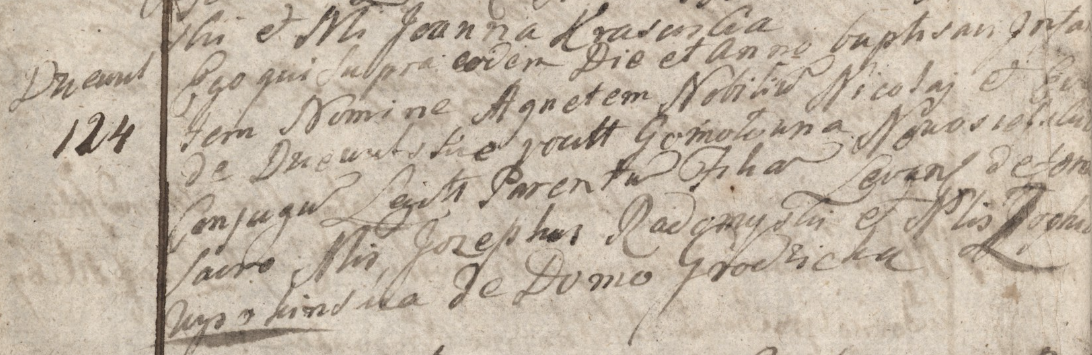
\includegraphics[width=1.0\linewidth]{
        1766_Agnieszka_Nowosielska_Gomołówna_akt_narodzin_parafia_Zbuczyn_wpis_124.png}
    \captionsetup{format=hang}
    \caption{Akt chrztu Agnieszki Nowosielskiej - par. Zbuczyn 1766~rok 
    (124/1765-1772) \cite{par_zbuczyn4}.}
    \label{fig:anowosielska_1766}
\end{figure}

Ostatnią osobą urodzoną w~Dziewulach, w~której akcie chrztu pojawia się 
przydomek zaczynający się od przedrostka \enquote{Gom}, jest Agnieszka 
Nowosielska (ur. 1766~r. - patrz: ryc. \ref{fig:anowosielska_1766}), córka 
Mikołaja i Ewy. Z~aktu jej chrztu wynika, iż jej matką była Ewa Dziewulska 
Gomołówna, która była prawdopodobnie córką wspominanego wcześniej Macieja 
Dziewulskiego Gomolika. Wygląda na to, że Ewa Dziewulska Gomoła była ostatnią 
przedstawicielką swojej gałęzi rodziny Dziewulskich w~Dziewulach. Wraz z~nią, 
gałąź ta zaniknęła całkowicie w~Dziewulach - w~metrykach parafialnych parafii 
zbuczyńskiej z~kolejnych kilkudziesięciu lat (po 1766~roku), przydomki / 
nazwiska Gomolak / Gomolik / Gomoła / Gomuła nie pojawiają się już w~ogóle. 
Najbardziej prawdopodobną przyczyną tego zaniknięcia było opuszczenie Dziewul 
przez rodziny posługujące się przydomkiem rozpoczynającym się od przedrostka 
\enquote{Gom} i~przeprowadzka do innej miejscowości, gdzie udało się im się 
podjąć pracę zarobkową w~charakterze najemnych chłopów / pracowników dworu. 
Nie byłoby to nic nadzwyczajnego w~tamtych czasach, gdyż jak zostało 
wspomniane na początku bieżącego rozdziału, już w~połowie XVI~wieku drobna 
szlachta zagrodowa mieszkająca w~Dziewulach nie posiadała często własnych 
chłopów i~sama zajmowała się uprawą roli. Wraz z~zanikaniem w~Dziewulach 
Dziewulskich posługujących się przydomkami Gomolak / Gomolik / Gomoła / 
Gomuła, w~jednej z~okolicznych parafii - w~Wilczyskach, a~konkretnie we wsi 
Wnętrzne, w~tym samym czasie, zaczęli się pojawiać chłopi o~nazwiskach 
Gomolak / Gomoła / Gomuła, którzy nie urodzili się na terenie wilczyńskiej 
parafii, a~przynajmniej nie sposób jest odnaleźć tam aktów urodzenia prawie 
żadnego z~nich.